\section{Introdução e Justificativa}
\label{sec:int}

Jogos de interpretação multijogador massivos surgiram de uma categoria de jogos de mesa baseados em representação de personagens nomeado como \textit{Role-Playing Game} (RPG), exemplos de \textit{Dungeon and Dragons} \cite{tsr1980dungeons}. A principal característica desse estilo de jogo é a comunicação e representação virtual de um mundo onde cada jogador pode interagir com objetos virtuais ou outros jogadores, tendo como maior objetivo do jogo a resolução de problemas e desenvolvimento do personagem \cite{video_game_technologies}.

O mercado de jogos massivos vem crescendo desde 2012 \cite{new_york_times}, sendo 2016 um dos mais lucrativos até então segundo o site Statista \cite{statista_2016}. A sua projeção para 2018 é que sejam arrecadados mais de 30 bilhões de dólares americanos com essa categoria de jogos \cite{statista_2018}, um aumento de 20% a mais sobre o ano de 2016.

Se faz de extrema importância a pesquisa sobre este gênero para melhorar a qualidade de serviço e otimizar o transporte de dados entre o cliente e o serviço online. Um dos grandes problemas atuais é a escalabilidade e qualidade desses serviços, visto que temos que entregar um serviço escalável conforme a demanda de usuários sem perder tempo de resposta, tornando um serviço crítico e sensível a pequenas alterações e detalhes de sua implementação.

\begin{figure}[h]
\caption{Plot gráfico comparando o número de conexões ao decorrer de 11 dias
\cite{system_performance}.}
\centering
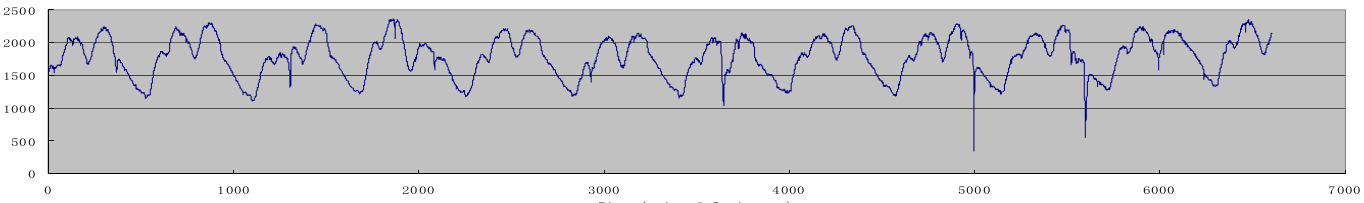
\includegraphics[width=1\textwidth]{img/connection_peer_hour.png}
\label{fig:conection_peer_hour}
\end{figure}

A Figura ~\ref{fig:conection_peer_hour} mostra um serviço de MMORPG utilizando 4 servidores distintos separados por um multiplexador. Pode-se perceber que existem picos próximos a 2250 conexões.

A análise realizada por \cite{system_performance} mostra um jogo de pequeno porte. Jogos de porte maior podem conter milhares de jogadores online simultaneamente. Um exemplo é o jogo RuneScape, a qual possui 90 mil jogadores online simultaneamente \cite{runescape_online_users}.
